% !TEX root = ../../main.tex

\chapter{Cost Estimation}

\label{chapter:cost-estimation}
In this chapter, we share the results of our experiments and explain how we used these results to build four different cost models. The \hyperref[sec:5-motivation]{first section} shows the results of the experiments, motivating why a cost model is necessary. In the \hyperref[sec:5-gpu-performance-analysis]{next section} the collected profiling metrics are aggregated and analyzed. In \autoref{sec:5-cost-models}, we talk about how we used the combined results, from the runtime and profiling experiments, to create the cost models. Each model is made for a specific purpose and offers different ways to solve the problem. This chapter aims to give a clear picture of how we ran the experiments and built the cost models from the results.

\section{Motivation}
\label{sec:5-motivation}
This section shows why there is a need for accurate cost estimation for choosing between factorization and materialization. We motivate in three stages. First the benefit of factorization is shown, second we show the impact of data \& model characteristics. By visualizing the performance ratio ($\frac{\text{Time}_M}{\text{Time}_F}$) against a range of independent variables we uncover the first trends that influence the F/M trade-off. Last, we show why GPUs are an important dimension to consider. All figures and values in this section are computed from the experiments with synthetic datasets, unless specified otherwise.

\subsection{Benefit of Factorization}
\begin{figure}[ht]
    \centering
    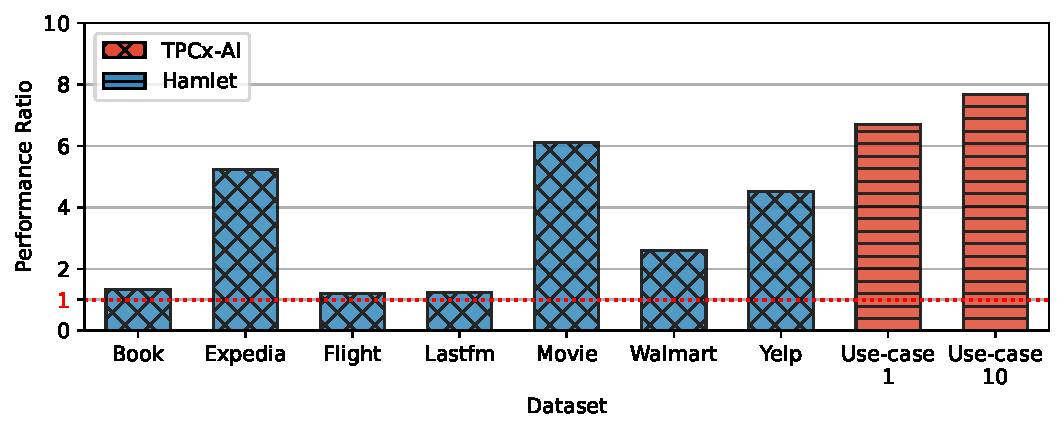
\includegraphics[width=\linewidth]{chapters/05_cost_estimation/figures/real_datasets_speedup.pdf}
    \caption[Performance gain with factorization on real datasets]{Average Performance ratio of ML models for positive cases ($\text{Time}_M > \text{Time}_F$), split per tested real dataset for.}
    \label{fig:5-real-perf-ratio}
\end{figure}

The goal of factorized ML is reducing the number of redundant operations performed during training of a model, to make this process more efficient, i.e., faster. We show the performance gain of factorization over materialization, on real datasets, in \autoref{fig:5-real-perf-ratio}. This shows that exploring factorization is beneficial, as for those cases where it is faster (which is $18\%$ of the tested cases on real datasets), the average speedup is $5.1\times$. In the most extreme cases the training time is reduced by more than $20$ seconds, a reduction by a factor of $27$. In scenarios where training occurs often, e.g., during hyperparameter optimization or online learning this can lead to significant time savings.

% We group the Data and Model characteristics as they both influence the actual computations being executed. The hardware characteristics influence how these computations are carried out on the hardware and are discussed separately. 

\subsection{Data \& Model Characteristics}
We show the impact of various data characteristics on the performance ratio in \autoref{fig:5-complexity-ratio-vs-data-chars}. The figure shows a slight negative correlation between performance ratio and sparsity of target table $T$. The second column shows more insight into the relation between performance and sparsity. It shows that when the sparsity ratio is low, i.e., compared to the base tables $S_k$, $T$ has more zero values, factorization is likely slower than materialization. The right-most plots show that a higher complexity ratio ($\frac{M_{FLOPs}}{F_{FLOPS}}$) is likely to lead to factorization being the training method. This is in line with the intuition that factorization is beneficial when it saves redundant computations. Important to note is that the correlation between these data characteristics and the speedup factorization brings is not as clear when we use GPUs for computation. This is likely due to the fact that the computations are not compute-bound but memory-bound. This is discussed further in the next section.

\begin{figure}[ht]
    \centering
    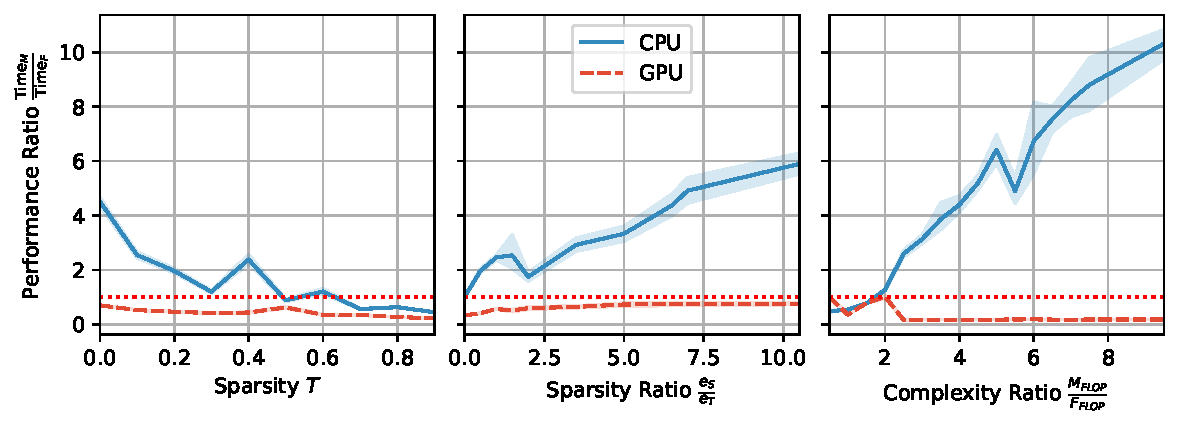
\includegraphics[width=\linewidth]{chapters/05_cost_estimation/figures/motivation_perf_ratio_vs_data_chars.pdf}
    \caption[Performance ratio for various data characteristics]{Performance ratio against various data characteristics. Broken down by compute type (CPU/GPU) and operator type (ML models in the first row \& regular operators in the second). $99\%$ confidence interval shown as shaded area. The sparsity ratio is defined as the sparsity of the source tables $S_k, k\in[1,n]$ divided by the sparsity of target table $T$. Sparsity of $S$ is defined as the total non-zero values in the base tables divided by the total number of cells in the base tables, $\frac{\sum_{k=1}^{n} nnz(S_k)}{\sum_{k=1}^{n} r_{S_k} \times c_{S_k}}$. High sparsity ratio means the target table is relatively sparser than the source tables.}
    \label{fig:5-complexity-ratio-vs-data-chars}
\end{figure}

\subsection{Hardware Characteristics}
The hardware used for computation impacts the runtime of a program, but here we show it also impacts the F/M trade-off. Different compute unites (i.e., CPU or GPU type) have a different decision boundary for when to use Factorization over Materialization. This is shown in \autoref{fig:5-gpu-characteristics}. Differing hardware impacts the performance ratio differently per operator. For example, the (mean$\pm$std.) performance ratio of transposed Left Matrix Multiplication on the P100 is $3.03\pm2.70$, while on the V100 it is slightly lower with $2.32\pm2.21$. But, for Left (scalar) multiplication the V100 has the higher performance ratio of $0.21\pm0.04$, against the P100's lower $0.19\pm0.05$.

\begin{figure}[ht]
    \centering
    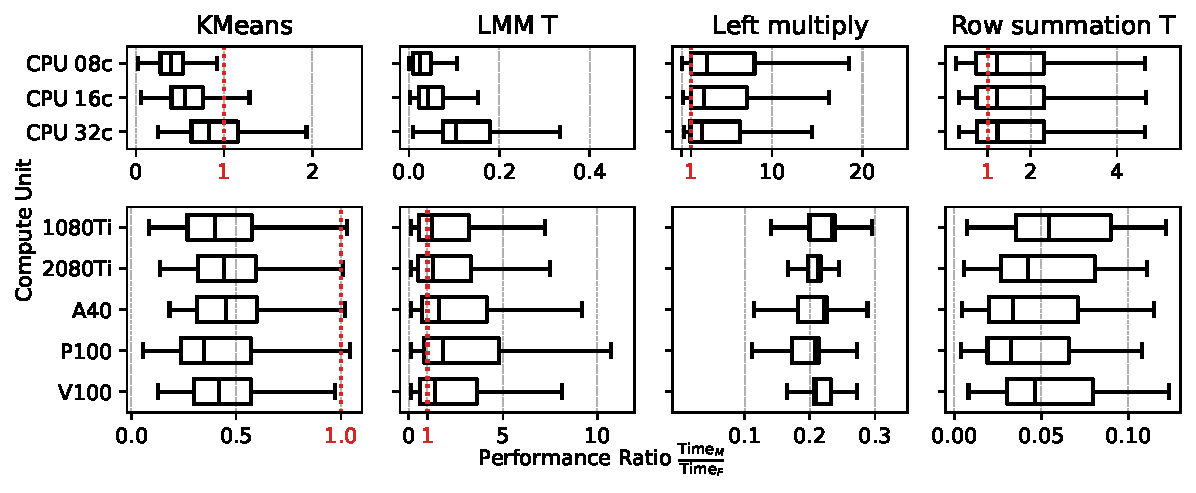
\includegraphics[width=\linewidth]{chapters/05_cost_estimation/figures/motivation_speedup_per_operator_per_gpu.pdf}
    \caption[Performance ratio plotted against hardware]{Performance ratio, of various operators on synthetic data, against hardware. The performance ratio is shown to be affected by hardware choice.}
    \label{fig:5-gpu-characteristics}
\end{figure}

\begin{table}[ht]
    \centering
    % LTeX: enabled=false
\begin{tabular}{lrrrr}
\toprule
Compute Unit & Mean & Std. Dev. & Count & \% with Speedup \\
\midrule\midrule
CPU 08c & 1.27 & 0.25 & 172 & 1.78\% \\
CPU 16c & 1.32 & 0.34 & 579 & 5.99\% \\
CPU 32c & 1.48 & 0.46 & 2873 & 29.74\% \\
1080Ti & 2.27 & 1.60 & 432 & 4.47\% \\
2080Ti & 1.87 & 1.09 & 425 & 4.40\% \\
A40 & 2.00 & 1.20 & 392 & 4.06\% \\
P100 & 2.52 & 1.84 & 461 & 4.77\% \\
V100 & 1.95 & 1.13 & 404 & 4.18\% \\
\bottomrule
\end{tabular}

    \caption[Performance ratio of ML models for cases where factorization has positive impact.]{Mean performance ratio of ML models for cases where Factorization is preferred over Materialization (speedup > 1). This shows hardware choice is a large factor in when to choose Factorization over Materialization.}
    \label{tab:5-speedup-per-gpu}
\end{table}

If we investigate these differences between GPUs further we see that, for cases where Factorization is preferred over Materialization ($\text{Time}_F < \text{Time}_M$), there are large differences between the GPUs. Both the mean performance ratio, and the count of cases where F is faster than M varies greatly, as shown in \autoref{tab:5-speedup-per-gpu}. This shows that the choice of hardware is a large factor in when to choose Factorization over Materialization.

Another interesting observation can be seen when comparing the performance ratio against the complexity ratio \cite{schijndel_cost_estimation}, for different hardware settings. As explained in \autoref{sec:3-cost-estimation-for-factorized-ml} the complexity is defined as the number of FLOPs needed to perform the operation. The ratio is defined as the complexity of the factorized case divided by the complexity of the materialized case. Thus, per \cite{schijndel_cost_estimation}, the higher this ratio the more beneficial it is to use factorization. However, our experiments show that while this is the case for a lot of operators on CPU, when performing the computations on GPUs this is not always the case. This is shown in \autoref{fig:5-complexity-ratio-vs-performance-ratio}.

\begin{figure}[ht]
    \centering
    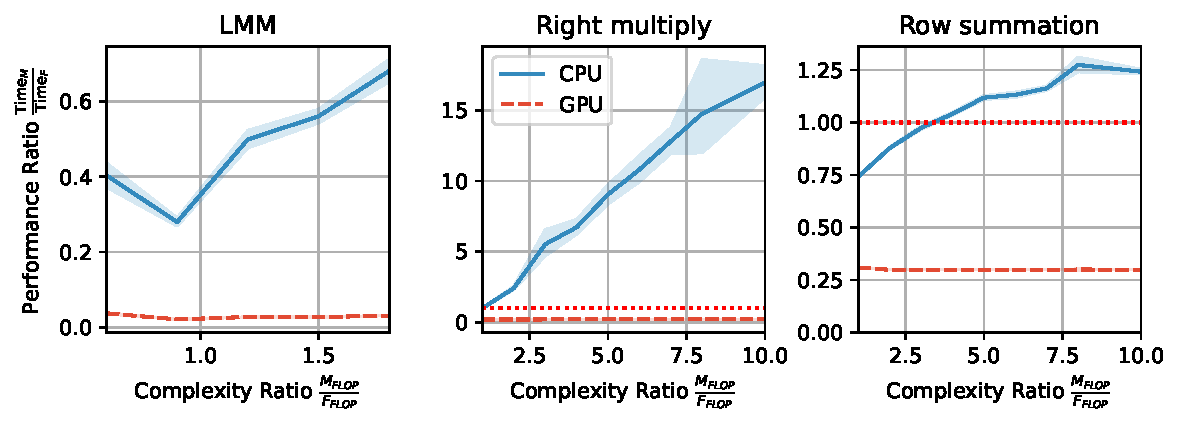
\includegraphics[width=\linewidth]{chapters/05_cost_estimation/figures/motivation_speedup_complexity_ratio.pdf}
    \caption[Performance ratio plotted against complexity ratio]{Performance ratio, of various operators on synthetic data, against complexity ratio, broken down by CPU and GPU. 95\% Confidence interval shown as shaded area. Where a lot of operators show clear correlation between the complexity ratio and the performance ratio on CPU, this is not the case for GPU.}
    \label{fig:5-complexity-ratio-vs-performance-ratio}
\end{figure}

\todo{Write last thing about GPU and why the correlations in \autoref{fig:5-complexity-ratio-vs-data-chars} are not as clear as for CPU.}

\section{GPU Performance Analysis}
\label{sec:5-gpu-performance-analysis}
Following NVIDIA's advice, a fitting way to estimate the runtime of a GPU program is to compute $max(T_{mem}, T_{math})$. In this formula $T_{mem}$ is the time it takes to transfer data to and from GPU memory, and $T_{math}$ is the time it takes to perform the actual computations. This is in line with the fact that the memory throughput of a GPU is much higher than that of a CPU, and thus the computations are often memory-bound. In this section we show whether this is the case for our experiments, and how we can use this to estimate the runtime of a program.

\todo{Describe \autoref{fig:5-profiling-mem-vs-compute}}

\begin{figure}[h]
    \centering
    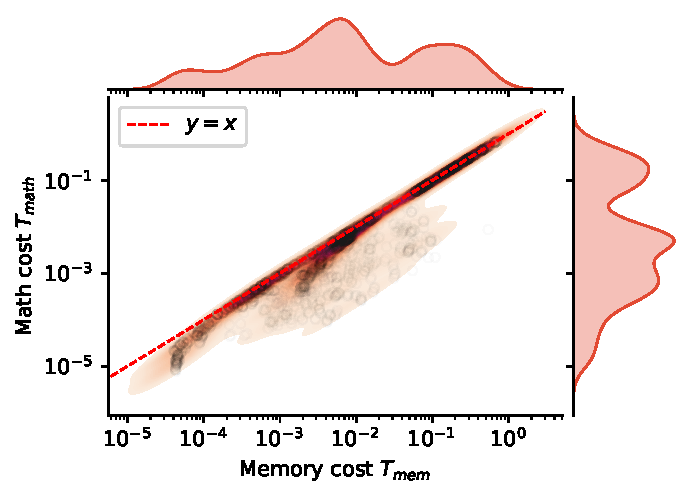
\includegraphics[width=0.5\linewidth]{chapters/05_cost_estimation/figures/profiling-mem-vs-compute.pdf}
    \caption[Memory cost vs math cost of profiled scenarios]{Memory cost vs math (compute)cost of profiled scenarios. The memory cost is computed as the total number of bytes read and written to memory divided by the measured average memory bandwidth. The math cost is the number of cycles the Streaming Multiprocessors were active divided by the measured average SM frequency.}
    \label{fig:5-profiling-mem-vs-compute}
\end{figure}


\todo{Add this section showing things like ops:bytes ratio differences between GPUs \& operators?
    % results/full_1/analytical_model/analytical.ipynb}
    \begin{enumerate}
        \item Something like figure 10 in \cite{tvm}. \textbf{Roofline chart.}
        \item Show that \\ \texttt{(dram\_bytes\_read\_sum + dram\_bytes\_write\_sum) / memory\_throughput\_byte\_weighted\_mean} is a good estimator for duration.
    \end{enumerate}
}

\section{Cost Models}
\label{sec:5-cost-models}
\todo{Detail the full process going from data to Cost model, what features where used, and what is the inner architecture?\\Show each of the factors is significant. Data, Hardware, Model parameters.\\Show R2 score to compare between models.}

\subsection{Feature Engineering}
\label{sec:5-feature-engineering}
\todo{
    Data Preprocessing steps
    \begin{enumerate}
        \item Collection of data characteristics
        \item Complexity
        \item ratios: complexity, sparsity
        \item Memory costs from profiling metrics
        \item Computation costs from profiling metrics
    \end{enumerate}
    Finally show schema of the final dataset used for training the models.
}

\begin{figure}[ht]
    \centering
    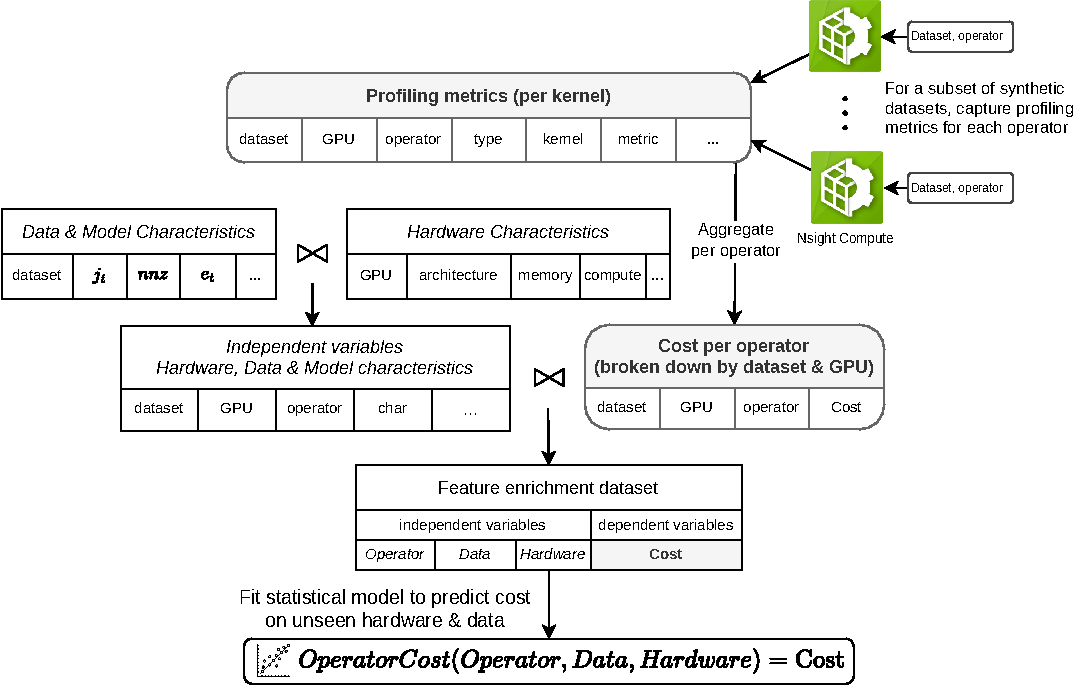
\includegraphics[width=\linewidth]{chapters/05_cost_estimation/figures/feature-engineering.pdf}
    \caption[Feature enrichment workflow]{Workflow of enriching the collected data with additional features from the profiling experiments. Items related to these profiling experiments are \textbf{bolded}, while the features from the data, model \& hardware characteristics are \textit{italicized}.}
    \label{fig:5-feature-enrichment}
\end{figure}

\subsection{Analytical}
\begin{figure}[ht]
    \centering
    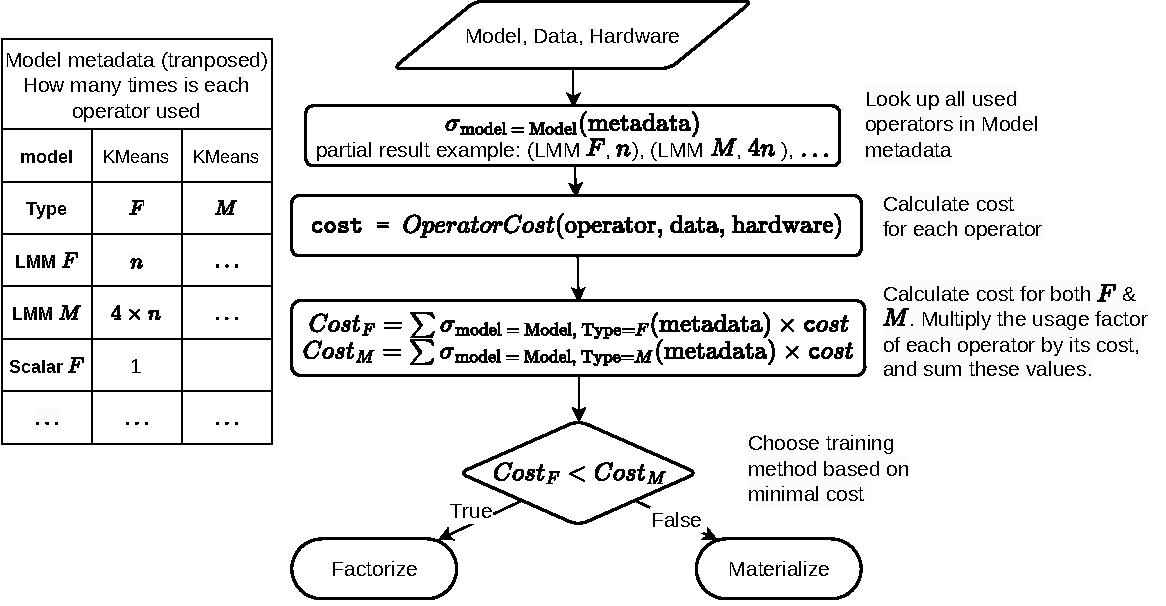
\includegraphics[width=\linewidth]{chapters/05_cost_estimation/figures/analytical-architecture.pdf}
    \caption[Analytical Estimator Architecture]{Architecture of the Analytical Estimator. Shows the control flow of inputs to a final decision on whether to use factorization or materialization. $OperatorCost$ is the function as defined in \autoref{fig:5-feature-enrichment}.}
    \label{fig:5-analytical-architecture}
\end{figure}

\subsection{Statistical}
The goal for this statistical estimator is to still be explainable, while providing higher performance than the hand tuned decision rules from related works. We use a variety of models, which all use Linear Regression at their core. We start with a singular regressor, and, by fine-tuning, end up at more complex models, with ensembles of linear regression models. The architecture of each of the statistical models is explained in \autoref{fig:5-statistical-architecture}.


\todo{
    \begin{enumerate}
        \item Linear Regression
        \item Difference with Analytical: predict time\_saved instead of runtime for both F and M.
              % \item For each fitted regressor we use Recursive feature elimination with cross-validation to select features \cite{rfecv}.
        \item Start with the simplest single linear regression model, continue to ensembles.
    \end{enumerate}
}

\begin{figure}[ht]
    \centering
    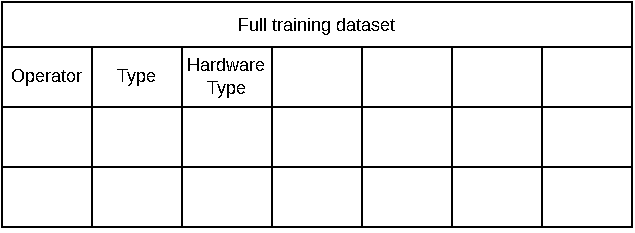
\includegraphics[width=\linewidth]{chapters/05_cost_estimation/figures/statistical-architecture.pdf}
    \caption[Statistical Estimator Architecture]{Architecture of the Statistical Estimator. Shows how the data, and estimators are split for each model. The final split-level belonging to each respective model is colored in the same color. For STAT.5 we show the linear regression ensemble fit to the data. For clarity, we leave this out for the other models. Three dots ($\boldsymbol{\ldots}$) denote some values were left out to prevent clutter.}
    \label{fig:5-statistical-architecture}
\end{figure}

\subsubsection*{STAT.1 Linear Regressor Fit to Full Training Set}
The first linear regressor is trained on the full training set, which includes all operators. The rationale behind this approach is that there is likely a relationship between the performance of individual operators and the performance of the models in which they are used. By training the regressor on the full set of operators, we aim to capture these relationships and use them to improve the accuracy. This model predicts the time saved by choosing factorization over materialization.

\subsubsection*{STAT.2 Linear Regressor Fit to Model Runtimes}
The second linear regressor is trained on the runtimes of the models. With this model we find whether including the operators adds utility. Like STAT.1, this model predicts the time saved by choosing factorization over materialization.

\subsubsection*{STAT.3 Separate Regressors for F and M}
This model is an ensemble of two linear regressors, one for factorization and one for materialization. By training separate regressors for factorization and materialization, we aim to capture the relationships between independent variables and runtime more explicitly than is done by the previous models. Each internal regressor predicts the runtime of the scenario under test, and the final prediction is which is predicted to be faster.

\subsubsection*{STAT.4 Separate Regressors for each Model Type}
Much like STAT.3 this estimator is also a combination of multiple inner regressors. However, instead of having one regressor for each factorization and materialization, we have one regressor for each model type. This is done to capture the differences in the relationships between independent variables and runtime for different model types. Like the first two models, this model predicts the time saved by choosing factorization over materialization (by predicting whether time is saved by choosing F).

\subsubsection*{STAT.5 Separate Regressors CPU and GPU}
In previous sections we have shown that the choice of hardware plays a large factor in the trade-off we are researching, therefore it is likely there are differences in the relationships between independent variables and runtime between CPU and GPU. A single linear regression model is likely unable to capture these differences. Therefore, we test the performance of a couple of estimators, one which is only fit to CPU scenario's, and one which is only fit to GPU scenario's.

\subsubsection*{STAT.6 Separate Regressors for F, M and Model Type}
The last version of the statistical model we created is a combination of STAT.4 and STAT.3. By training separate regressors for every combination of factorization, materialization and model type, we allow the models to capture differences between the groups more freely.

\subsubsection*{STAT.7 Separate Regressors Each Dimension}
The last, most granular, ensemble is one that has a separate regressor for each combination of factorization, materialization, model type and hardware. This is done to capture the differences in the relationships between independent variables and runtime for each combination of the dimensions.


\subsubsection{Statistical Model Evaluation}
\todo{Text to go with \autoref{fig:5-statistical-model-evaluation}.}

\begin{figure}[ht]
    \centering
    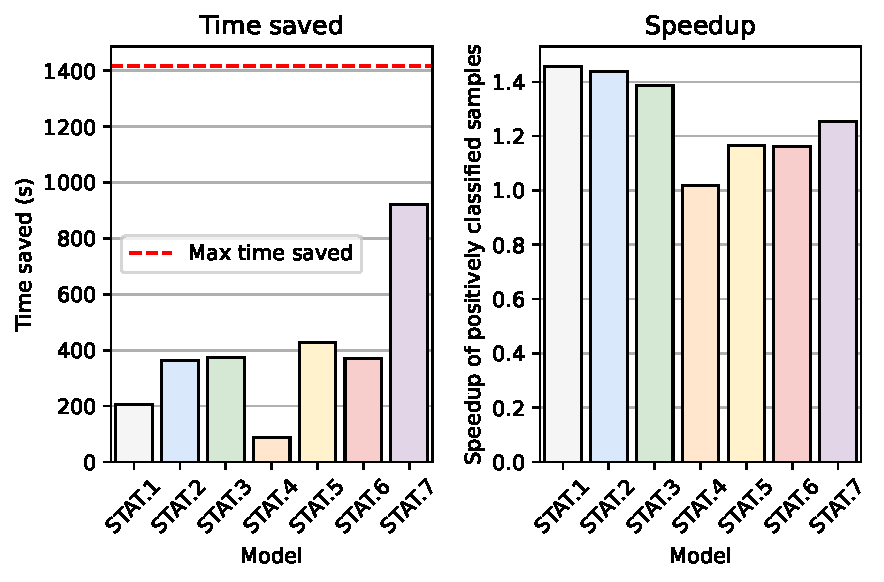
\includegraphics[width=\linewidth]{chapters/05_cost_estimation/figures/stat-models-compare.pdf}
    \caption[Statistical Model Evaluation]{Evaluation of the statistical models on the test set (synthetic data, only models). The first two plots show statistics of those scenarios where the estimator predicts factorization to be faster. The last plot shows the time saved when using this estimator, as a fraction of the total to-be-saved time (by a perfect estimator).}
    \label{fig:5-statistical-model-evaluation}
\end{figure}

\subsection{Deep Learning}

\subsection{Hybrid}

\subsection{Meta-results}
\todo{Inference speed, training time.}
